\section{Results}
\label{sec:results}

We organize results around five questions: (1) whether the spectral advantage is family-level and how it depends on architecture (\S\ref{sec:main_results}), (2) whether it persists with longer training (\S\ref{sec:convergence_efficiency}), (3) what layer-wise mechanisms underlie it (\S\ref{sec:spectral_analysis}), (4) whether it generalizes to modern training recipes (\S\ref{sec:recipe_robustness}), and (5) whether the advantage is attributable to spectral preconditioning itself (\S\ref{sec:ablation}).

%% ===================================================================
\subsection{Spectral Advantage: Magnitude and Architecture Dependence}
\label{sec:main_results}
\label{sec:gap_magnitude}

If spectral optimizers succeed by exploiting weight-matrix structure, their advantage should be universal across architectures but variable in magnitude.
Table~\ref{tab:main_results} confirms this prediction: Muon outperforms AdamW across all nine architecture-dataset pairs, with gaps ranging from $+5.9$\,pp (ResNet-50/Tiny-ImageNet) to $+24.3$\,pp (ConvNeXt-T/ImageNet-100), as visualized in Figure~\ref{fig:overview}(b).
Multi-seed variance is low ($0.05$--$2.17$\,pp; Appendix Table~\ref{tab:multi_seed}), confirming that observed gaps substantially exceed run-to-run noise.
All nine Muon-AdamW gaps are statistically significant after Holm--Bonferroni correction (Welch's $t$-test, $p < 0.02$, Cohen's $d > 10$ in every pair), confirming that the advantage is not attributable to seed variance.
The 20-epoch budget serves as a controlled stress test of optimizer-intrinsic convergence capacity, independent of augmentation and scheduling.
Our main comparison uses a fixed minimal recipe to isolate optimizer effects; \S5.4 and Appendix show the advantage persists under enhanced recipes and independent per-optimizer LR sweeps, though fully architecture-optimized protocols may narrow the gap.

\begin{table}[t]
\centering
\caption{Best validation accuracy (\%) at 20 epochs. Multi-seed results ($\pm$ std) where available; $^\dagger$single-seed (seed\,=\,42). Bold = best per column. Gap = best spectral $-$ AdamW in pp. $^\ddagger$Muon$-$AdamW only (SOAP/Shampoo evaluated on CIFAR-100 only). Significance: Welch's $t$-test with Holm--Bonferroni correction across 2--4 seeds. $^{*}p<0.05$, $^{**}p<0.01$, $^{***}p<0.001$. For Tiny-ImageNet and ImageNet-100, where only Muon is evaluated among spectral methods, the gap is Muon$-$AdamW.}
\label{tab:main_results}
\vspace{-0.5em}
\setlength{\tabcolsep}{4pt}
\small
\begin{tabular}{@{}llccc@{}}
\toprule
Dataset & Optimizer & ResNet-50 & DeiT-S & ConvNeXt-T \\
\midrule
\multirow{6}{*}{CIFAR-100}
  & Shampoo & \textbf{78.25}{\scriptsize$\pm$0.18} & 63.53{\scriptsize$\pm$0.05} & 70.57{\scriptsize$\pm$0.29} \\
  & SOAP  & 77.28{\scriptsize$\pm$0.20} & \textbf{65.45}{\scriptsize$\pm$0.18} & 74.40{\scriptsize$\pm$0.43} \\
  & Muon  & 76.88{\scriptsize$\pm$0.27}$^{***}$ & 62.67{\scriptsize$\pm$0.41}$^{***}$ & \textbf{74.62}{\scriptsize$\pm$0.15}$^{**}$ \\
  & AdamW & 67.85{\scriptsize$\pm$0.17} & 52.33{\scriptsize$\pm$0.34} & 58.54{\scriptsize$\pm$2.17} \\
  & SGD   & 69.50{\scriptsize$\pm$0.39} & 43.98{\scriptsize$\pm$0.48} & 11.51$^\dagger$ \\
\midrule
  & \textit{Gap} & \textbf{+10.40} & \textbf{+13.12} & \textbf{+16.08} \\
\midrule
\multirow{4}{*}{Tiny-ImageNet}
  & Muon  & \textbf{62.66}{\scriptsize$\pm$0.32}$^{***}$ & \textbf{48.02}{\scriptsize$\pm$0.21}$^{***}$ & \textbf{58.92}{\scriptsize$\pm$0.19}$^{***}$ \\
  & AdamW & 56.76{\scriptsize$\pm$0.45} & 40.33{\scriptsize$\pm$0.42} & 43.92{\scriptsize$\pm$0.29} \\
  & SGD   & 60.04$^\dagger$ & 34.22$^\dagger$ & 9.49$^\dagger$ \\
\midrule
  & \textit{Gap$^\ddagger$} & \textbf{+5.90} & \textbf{+7.69} & \textbf{+15.00} \\
\midrule
\multirow{4}{*}{ImageNet-100}
  & Muon  & \textbf{61.97}{\scriptsize$\pm$0.25}$^{**}$ & \textbf{37.04}{\scriptsize$\pm$0.38}$^{***}$ & \textbf{57.83}{\scriptsize$\pm$0.21}$^{**}$ \\
  & AdamW & 50.50{\scriptsize$\pm$0.76} & 26.12{\scriptsize$\pm$0.10} & 33.53{\scriptsize$\pm$1.51} \\
  & SGD   & 50.06$^\dagger$ & 20.38$^\dagger$ & 6.77$^\dagger$ \\
\midrule
  & \textit{Gap$^\ddagger$} & \textbf{+11.47} & \textbf{+10.92} & \textbf{+24.30} \\
\bottomrule
\end{tabular}
\vspace{-0.5em}
\end{table}

\paragraph{Spectral Family Comparison on CIFAR-100.}
A critical question for interpretation is whether the advantage is specific to Muon's Newton--Schulz mechanism or shared across spectral methods.
We evaluate SOAP~\cite{vyas2025soap} and Shampoo~\cite{gupta2018shampoo} on CIFAR-100 under the same protocol (Table~\ref{tab:main_results}; full comparison in Appendix Table~\ref{tab:spectral_comparison}).
SOAP matches Muon within noise on ResNet-50 and ConvNeXt-T and outperforms it on DeiT-S ($+3.10$\,pp, $p < 0.001$).
Within the spectral optimizer class, Shampoo leads on ResNet-50 ($+1.37$\,pp over Muon), SOAP on DeiT-S ($+3.10$\,pp, $p{<}0.001$), and Muon on ConvNeXt-T ($+4.05$\,pp), with each architecture favoring a different spectral variant.
All spectral optimizers outperform AdamW by $+9$--$+16$\,pp on CIFAR-100, with intra-family differences ($1.4$--$4.1$\,pp) approximately $4$--$8\times$ smaller than the spectral-AdamW gap, suggesting the benefit as a \emph{family-level} trend on CIFAR-100, with intra-class variation (Appendix~\ref{sec:hyperparams}).

\paragraph{Architecture dependence.}
Figure~\ref{fig:overview}(b) reveals a consistent ordering: ConvNeXt-T exhibits the largest gap at every dataset ($+16.08$, $+15.00$, $+24.30$\,pp), $1.2$--$2.5\times$ larger than the other architectures, while ResNet-50 shows the smallest.
ConvNeXt-T consistently shows the largest gap while ResNet-50 shows the smallest, a pattern consistent across all three spectral methods (Appendix Table~\ref{tab:spectral_comparison}). We discuss the mechanistic basis for this ordering in Section~\ref{sec:discussion}.

%% ===================================================================
\vspace{-0.3em}
\subsection{Persistence of the Spectral Advantage: 20 vs.\ 50 Epochs}
\label{sec:convergence_efficiency}

\begin{figure}[t]
\centering
\begin{minipage}[b]{0.48\textwidth}
    \centering
    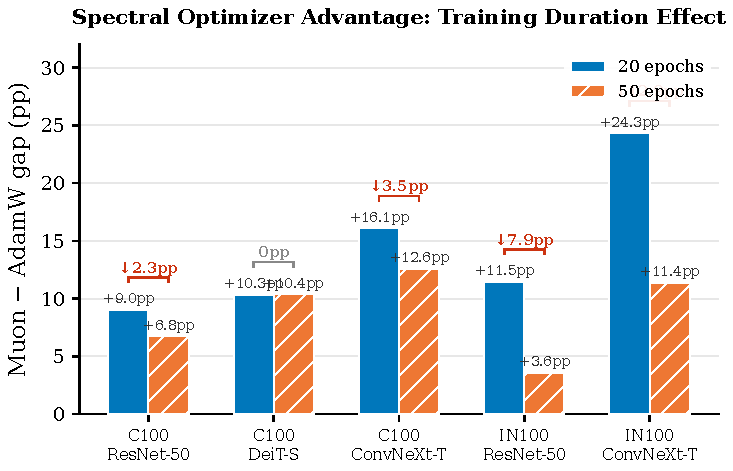
\includegraphics[height=3.6cm]{figures/fig2_gap_evolution.pdf}
    \vspace{-0.5em}
    \centerline{\small (a) Gap evolution from 20 to 50 epochs}
\end{minipage}
\hfill
\begin{minipage}[b]{0.42\textwidth}
    \centering
    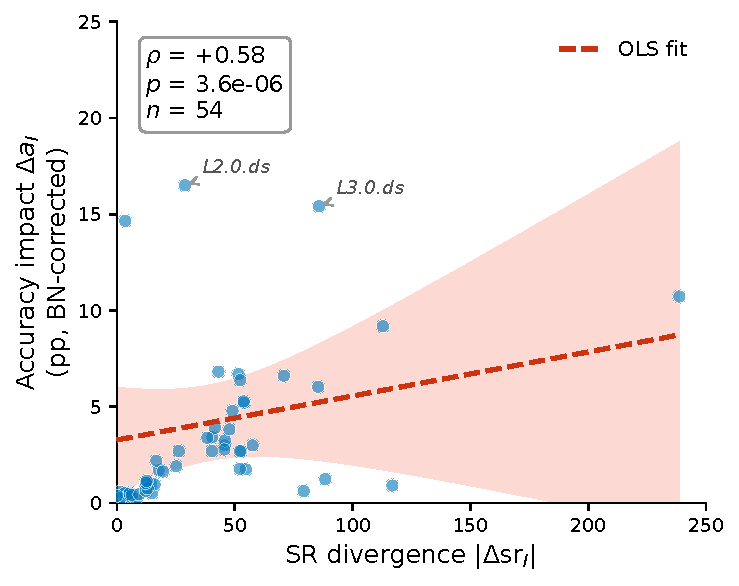
\includegraphics[height=3.6cm]{figures/fig3_spectral_divergence.pdf}
    \vspace{-0.5em}
    \centerline{\small (b) Layer-wise spectral divergence vs.\ accuracy impact}
\end{minipage}
\vspace{-0.5em}
\caption{Temporal persistence and mechanistic basis of the spectral advantage. (a) Muon-AdamW gap narrows on CNNs but persists on DeiT-S, revealing convergence-speed vs.\ solution-quality mechanisms. (b) On ResNet-50, stable-rank divergence correlates with weight-swap accuracy impact ($\rho = +0.58$, $p = 3.6 \times 10^{-6}$), indicating broad spectral reshaping across layers.}
\label{fig:gap_evolution}
\label{fig:sign_reversal}
\label{fig:combined_gap_spectral}
\vspace{-1em}
\end{figure}

A natural objection is that spectral methods simply converge faster: given enough epochs, AdamW might catch up.
We extend training to 50 epochs on CIFAR-100 and ImageNet-100 (Table~\ref{tab:gap_narrowing}; Figure~\ref{fig:gap_evolution}; epoch-level details in Appendix Table~\ref{tab:gap_evolution}).

\begin{table}[t]
\centering
\caption{Gap decomposition from 20 to 50 epochs (best validation accuracy throughout). $\Delta$Gap${}={}$50ep gap$-$20ep gap. Superscripts denote seed count: $^{(k)}$ = $k$-seed mean; $^\dagger$ = single seed (seed\,=\,42). IN100 AdamW seed\,=\,42 used $\text{lr}{=}3{\times}10^{-4}$ (vs.\ $3{\times}10^{-3}$ for other seeds); a verification run confirmed identical accuracy at both rates. All gaps are Muon $-$ AdamW.}
\label{tab:gap_narrowing}
\vspace{-0.5em}
\small
\footnotesize
\setlength{\tabcolsep}{3pt}
\begin{tabular}{@{}lccrrr@{}}
\toprule
Setting & 20ep gap & 50ep gap & $\Delta$Gap & Muon $\Delta$ & AdamW $\Delta$ \\
\midrule
C100 ResNet-50   & +9.03$^{(4)}$  & +6.76$^{(3)}$  & $-$2.27  & +0.89 & +3.16 \\
C100 DeiT-S      & +10.34$^{(4)}$ & +10.37$^{(3)}$ & +0.03  & +0.24 & +0.21 \\
C100 ConvNeXt-T  & +16.08$^{(4)}$ & +12.60$^{(3)}$  & $-$3.48  & $-$0.03 & +3.45 \\
IN100 ResNet-50  & +11.47$^{(4)}$ & +3.56$^\dagger$  & $-$7.91  & +0.27 & +8.18 \\
IN100 ConvNeXt-T & +24.30$^{(4)}$ & $\approx$+11.37$^\dagger$ & $\approx$$-$12.93 & +0.52 & +13.45 \\
\bottomrule
\end{tabular}
\vspace{-0.5em}
\end{table}

The answer is architecture-dependent.
On ResNet-50, AdamW gains $+3.16$\,pp while Muon gains $+0.89$\,pp, narrowing the gap from $+9.03$ to $+6.76$\,pp, a convergence-speed difference.
On DeiT-S, both gains are negligible ($<0.25$\,pp) and the gap is unchanged ($+10.37$ vs.\ $+10.34$\,pp), indicating a genuine solution-quality advantage.
On ConvNeXt-T, the gap narrows from $+16.08$ to $+12.60$\,pp as AdamW improves while Muon stays flat.
The pattern reveals two mechanisms: \emph{convergence speed} on CNNs (gap narrows but remains substantial) and \emph{solution quality} on transformers (gap unchanged, both optimizers plateau early at different solutions).
Spectral methods incur 5--22\% per-epoch overhead but achieve equivalent accuracy in $\leq$20 epochs vs.\ $\geq$50 for AdamW, yielding net $\geq$2$\times$ wall-clock savings (Appendix Table~\ref{tab:wallclock}).

%% ===================================================================
\vspace{-0.5em}
\subsection{Mechanistic Analysis: Architecture-Dependent Correlation and Normalization Dependence}
\label{sec:spectral_analysis}
\label{sec:sgd_failure}

The preceding sections establish \emph{that} spectral methods outperform across architectures; we now investigate \emph{where} in the network this advantage arises and \emph{why} it depends on normalization type.

\paragraph{Layer-wise weight swap reveals architecture-dependent correlation.}
Weight swap experiments (Section~\ref{sec:method}) show that Muon's advantage is near-universal on ResNet-50 (94.3\% of layers beneficial) but selective on DeiT-S (51.7\%).
The Spearman correlation between per-layer stable rank divergence $\Delta \mathrm{sr}_l$ and per-layer Muon benefit $\Delta a_l$ is positive on ResNet-50 ($\rho = +0.58$, $p = 3.6 \times 10^{-6}$, after BN recalibration), as visualized in Figure~\ref{fig:sign_reversal}.
On DeiT-S, the layer-wise benefit pattern shows no significant stable-rank correlation ($\rho \approx 0$, n.s.), contrasting with ResNet-50.
We report stable-rank divergence as our primary metric; the architecture-dependent correlation pattern is discussed further in Appendix~\ref{sec:metric_robustness}.

\paragraph{Architecture-dependent mechanisms.}
The correlation pattern reveals architecture-dependent mechanisms (Figure~\ref{fig:sign_reversal}).
On ResNet-50, the positive correlation ($\rho = +0.58$) means layers where Muon reshapes spectral structure most are where it helps most: \emph{broad spectral reshaping} across the network, with $94.3\%$ of layers benefiting.
Muon-trained ConvNeXt-T models exhibit $7.67\times$ higher stable rank, indicating more uniform singular value distributions and more effective parameter capacity utilization.
On DeiT-S, no significant stable-rank correlation is observed ($\rho \approx 0$, n.s.); the transformer mechanism remains to be characterized.

\begin{figure*}[t]
\centering
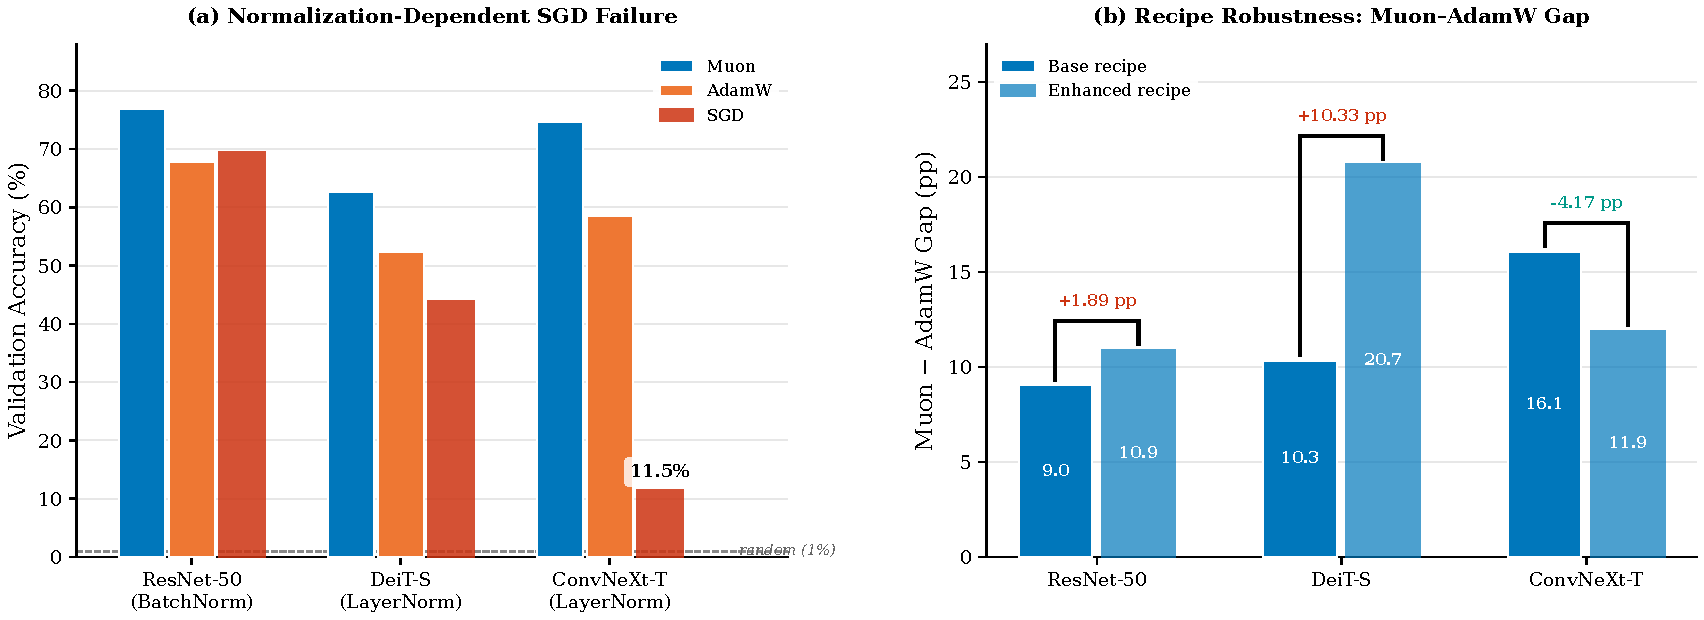
\includegraphics[width=0.88\textwidth]{figures/fig4_norm_recipe.pdf}
\caption{(a) Normalization-swap experiment on ResNet-50: replacing BatchNorm with LayerNorm collapses AdamW by ${\sim}17$\,pp and SGD degrades catastrophically (28.87\%, a $-40.6$ pp drop from BN), while Muon is preserved (+1.64\,pp). (b) Training recipe robustness: enhanced augmentation produces differential optimizer response across architectures, where Muon gains while AdamW is flat or declines.}
\label{fig:norm_recipe}
\label{fig:sgd_failure}
\label{fig:enhanced_recipe}
\end{figure*}

\paragraph{SGD failure as extreme normalization dependence.}
Figure~\ref{fig:sgd_failure} illustrates the most extreme manifestation: SGD collapses to near-random accuracy on ConvNeXt-T ($11.51\%$; Appendix~\ref{sec:convnext_sgd_analysis}) and degrades substantially on DeiT-S ($43.98\%$), while remaining competitive on batch-normalized ResNet-50 ($69.50\%$).
Independent verification confirms this is not a configuration error: lr sweep across 5 rates and weight-decay sanity check ($\Delta{=}{-}0.09$\,pp) both confirm SGD's genuine failure mode on this architecture.
Spectral methods resolve this coupling: Muon achieves $74.62\%$ on ConvNeXt-T where SGD fails, suggesting spectral preconditioning compensates for the landscape smoothing that batch normalization provides but layer normalization does not~\cite{santurkar2018how}.
This aligns with recent findings that sign descent properties, rather than noise handling, may explain adaptive methods's advantage on transformers~\citep{kunstner2024noise}.
The heavy-tailed gradient distribution in attention layers~\citep{zhang2020adaptive} provides a complementary explanation for SGD's failure.
Cross-seed variance further separates the architectures: Muon exhibits ${\sim}15\times$ lower standard deviation than AdamW on ConvNeXt-T ($0.15$ vs.\ $2.17$\,pp; Appendix Figure~\ref{fig:stability}), consistent with spectral preconditioning providing both accuracy and stability gains.

\paragraph{Normalization swap: dose-response evidence.}
\label{sec:norm_swap}
To isolate normalization as the mediating variable, we replace all BatchNorm layers in ResNet-50 with GroupNorm(1,$C$), equivalent to LayerNorm for convolutional layers~\cite{wu2018group,xiong2020layer}\footnote{GroupNorm(1,$C$) computes identical normalization statistics to LayerNorm; both use per-channel affine parameters in our implementation.}, while keeping all other hyperparameters fixed (Appendix~\ref{sec:normswap_details}).
Table~\ref{tab:norm_dose} summarizes the results.

\begin{table}[t]
\centering
\caption{Dose-response: accuracy (\%) under different normalization types on ResNet-50, CIFAR-100.}
\label{tab:norm_dose}
\footnotesize
\setlength{\tabcolsep}{3pt}
\begin{tabular}{lcccc}
\toprule
Optimizer & R50-BN & R50-GN(32) & R50-LN & BN$\to$GN32 $\Delta$ \\
\midrule
Muon    & 76.88 & 78.20 & 78.52 & $+1.32$ \\
SOAP    & 77.28 & 75.52 & ---   & $-1.76$ \\
Shampoo & 78.25 & 74.79 & ---   & $-3.46$ \\
AdamW   & 67.85 & 55.73 & 50.51 & $-12.12$ \\
SGD     & 69.50 & 23.90 & 28.87 & $-45.60$ \\
\bottomrule
\end{tabular}
\end{table}

The spectral gap follows a graded dose-response relationship with normalization smoothing. As smoothing decreases from BatchNorm through GroupNorm(32) to LayerNorm, AdamW accuracy degrades monotonically (67.85$\to$55.73$\to$50.51\%), while Muon remains invariant (76.88$\to$78.20$\to$78.52\%). SGD exhibits a binary failure mode: functional with BatchNorm (69.50\%) but catastrophically failing without it ($\sim$24--29\%).

\paragraph{Training stability under LayerNorm.}
SGD's cross-seed variance under LayerNorm ($\pm 8.17$\,pp) is $25\times$ higher than Muon ($\pm 0.32$\,pp), indicating that first-order optimization without BatchNorm is not merely less accurate but fundamentally unstable.
Muon's stability advantage extends beyond accuracy: cross-seed $\sigma$ ratio reaches $14.5\times$ on ConvNeXt-T, with spectral methods more stable in 6/9 configurations (Appendix Figure~\ref{fig:stability}).
This constitutes a controlled causal experiment: normalization type is the sole manipulated variable, establishing it as a mediating mechanism rather than a mere correlate.

%% ===================================================================
\vspace{-0.5em}
\subsection{Robustness to Training Recipe Variation}
\label{sec:recipe_robustness}

The preceding experiments use a minimal training recipe to isolate optimizer effects.
We evaluate an enhanced recipe adding warmup, Mixup~\cite{zhang2018mixup}, CutMix~\cite{yun2019cutmix}, RandAugment~\cite{cubuk2020randaugment}, and label smoothing~\cite{szegedy2016rethinking} on CIFAR-100 (Appendix~\ref{sec:enhanced_recipe_details}).

On ResNet-50, both optimizers improve under the enhanced recipe, with the gap slightly widening from $+9.03$ to $+10.92$\,pp (3-seed mean; Figure~\ref{fig:enhanced_recipe}).
The striking result is on DeiT-S: Muon benefits substantially ($+9.12$\,pp over baseline) while AdamW remains flat ($-1.21$\,pp), doubling the spectral gap from $+10.34$ to $+20.67$\,pp ($n{=}3$ seeds).
This \emph{differential optimizer response} is interpretable through the mechanistic framework of Section~\ref{sec:spectral_analysis}: spectral preconditioning operates on the full gradient matrix and more effectively exploits the richer gradient signal from advanced augmentation, whereas element-wise methods like AdamW cannot fully leverage this additional structure. Enhanced recipes (Mixup, CutMix, RandAugment) preserve the ranking: Muon leads by +5--8\,pp even under strong augmentation.

%% ===================================================================
\vspace{-0.5em}
\subsection{Ablation: Spectral Preconditioning vs.\ Parameter Grouping}
\label{sec:ablation}

A two-group AdamW configuration mirroring Muon's parameter routing achieves $66.36\%$ on ResNet-50 vs.\ Muon's $76.88\%$, comparable to single-group AdamW and far below Muon on both ResNet-50 ($+10.5$\,pp gap) and ConvNeXt-T ($+15.2$\,pp gap), confirming the advantage is attributable to spectral preconditioning, not dual learning-rate structure (Appendix~\ref{sec:ablation_details}).